\chapter[Marco Teórico]{\label{ch:marco-teorico}Marco Teórico}

\section{Sistemas Multi-core y OpenMP}

En este capitulo se describen los conocimientos básicos sobre programación multi-núcleos, programación en coprocesadores tales como programación en Intel Xeon Phi, programación en GPU y trabajos relacionados que dan base a esta tesis.\\
Actualmente las arquitecturas de los dispositivos personales están diseñadas con multiprocesadores o coprocesadores, desde un equipo de bolsillo como un celular (Smartphone) hasta un computador personal (notebook), esto quiere decir que los dispositivos cuentan con varios núcleos en una sola CPU (Unidad central de procesamiento) en el caso de multiprocesadores y con más de una CPU en el caso de un Coprocesador.\\ Imagen de referencia \ref{fig:plataforma}

\subsection{Threads}
Existen varias bibliotecas que permiten la programación en multi-hilos, con esto somos capaces de ejecutar hilos en paralelo, ejecutándose en un núcleo diferente.\\
Existen diferentes modelos y estándares que permiten la programación de múltiples hilos, tales como Pthreads \cite{libroPthreads}, TBB \cite{libroTBB} u OpenMP \cite{libroOpenMP}, en particular en esta tesis se selecciono el uso de la biblioteca OpenMP que fue desarrollada en 1997. Además es importante mencionar el hecho de que actualmente los compiladores en esta linea son bastante robustos, como tambien el hecho de que el equipo que gestiona OpenMP esta conformado por diferentes compañías (AMD, Intel, Sun Mycrosystem y otros) y no siendo gestionada por una sola, esto nos proporciona confianza.\\

\begin{figure}
\begin{center}
   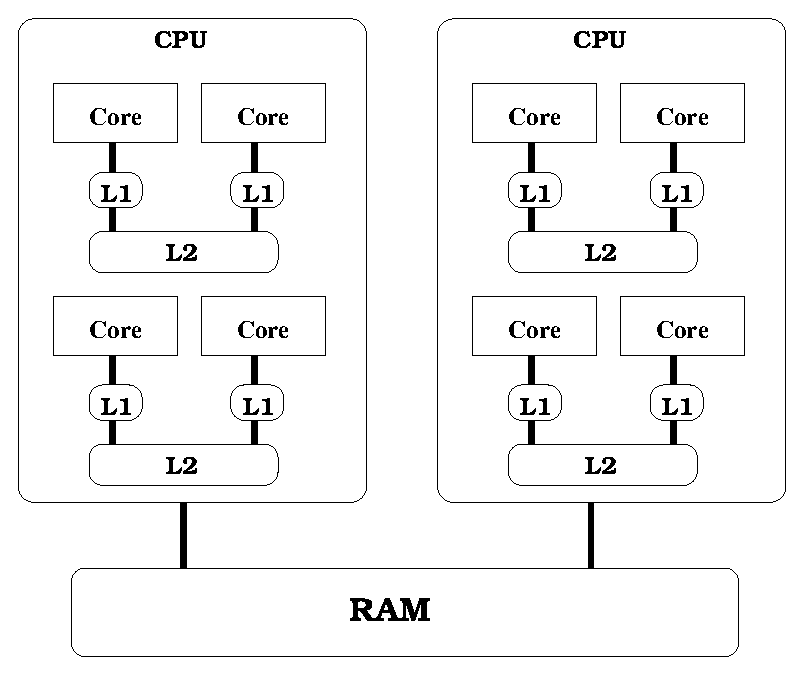
\includegraphics[scale=0.5]{fig/plataforma.eps}
\end{center}
\caption{\label{fig:plataforma}Plataforma multi-core.}
\end{figure}


\section{Coprocesadores} \label{cap:coprocesadores}

Un Coprocesador es utilizado para desligar funciones de la CPU, en esta linea existen desde coprocesadores matemáticos hasta coprocesadores gráficos, estos poseen características y especificaciones a ciertos tipos de operaciones, por ejemplo un coprocesador matemático solo esta desarrollado para revolver problemas aritméticos o afines al área esto quiere decir que pueden realizar operaciones matemáticas a una velocidad mayor que el procesador principal (CPU), a su vez un coprocesador gráfico esta diseñado en otra área. Estos proporcionan al hardware una aceleración en la operación solo cuando se ejecuta una tarea o software que se haya diseñado para aprovechar el coprocesador, las instrucciones para un coprocesador son diferentes que las instrucciones de una CPU de modo que existe un programa que detecta la existencia de un coprocesador y entonces se ejecutan las instrucciones escritas explícitamente para aquel coprocesador, por tanto existen diferentes lineas de coprocesadores en el mercado pero en esta tesis solo consideramos Intel Xeon Phi y GPU NVIDIA.

\subsection{Intel Xeon Phi}

El coprocesador Intel Xeon Phi \cite{xeonphi1} \cite{wange2014} \cite{xeonphila} consta de hasta 72 conectados en un anillo bidireccional de alto rendimiento en el chip. El coprocesador ejecuta un sistema operativo linux y es compatible con todas las principales herramientas de desarrollo de Intel como C / C ++, Fortran, MPI y OpenMP. El coprocesador se conecta a un procesador Intel Xeon (el host) a través del bus PCI Express (PCIe). Las propiedades más importantes de la arquitectura MIC se muestran en figura \ref{estructuraxeon}.\\

\textbf{Core:} El núcleo de la intel Xeon phi (Scalar Unit en la figura \ref{estructuraxeon}) es una arquitectura de orden (basada en la familia de procesadores Intel Pentium),Implementa instrucciones de recuperación y decodificación para 4 hilos (hardware) por núcleo. Las instrucciones vectoriales que posee el coprocesador Intel Xeon Phi, utiliza una unidad de punto flotante (VPU) dedicada, con un ancho de 512-bit, la que está disponible en cada núcleo. Un núcleo puede ejecutar dos instrucciones por ciclo de reloj, una en U-pipe y otra en V-pipe (no todos los tipos de instrucciones pueden ser ejecutadas por el V-pipe). Cada núcleo compone una interconexión en anillo mediante la CRI (Core Ring Interface).\\

\textbf{Vector Processing Unit (VPU):} La VPU incluye la EMU (Extended Math Unit), y es capaz de realizar 16
operaciones en punto flotante con precisión simple por ciclo, 16 operaciones de enteros de 32-bit por ciclo u
8 operaciones en punto flotante con precisión doble por ciclo.\\

\textbf{L1 Cache:} Tiene una caché L1 de 32KB para instrucciones y de 32KB para datos, asociativa de 8-vías,
con tamaño de línea de caché de 64 bytes. Tiene una latencia de cargado de 1 ciclo, que significa que un valor
entero cargado desde L1 puede ser usado en el siguiente ciclo por una instrucción entera (instrucciones vectoriales
tienen diferente latencia que las enteras).\\

\textbf{L2 Cache:} Cada núcleo posee 512KB de caché L2. Si ningún núcleo comparte algún dato o código, entonces el
tamaño total de la caché L2 es de 31 MB. Por otro lado, si todos los núcleos comparten exactamente el mismo
código y datos en perfecta sincronía, el tamaño total de la caché L2 sería solo de 512KB. Su latencia es de 11
ciclos de reloj.\\

\textbf{Ring:} Incluye interfaces y componentes, ring stops, ring turns, direccionamiento y control de flujo. Un coprocesador Xeon Phi tiene 2 de estos anillos, uno viajando en cada dirección (Figure \ref{estructuraxeon2}).\\

La Figura \ref{estructuraxeon2} ilustra una visión general de la arquitectura, donde se muestra como los núcleos están conectados con cachés coherentes mediante un anillo bidireccional de 115GB/sec. La figura también muestra una memoria GDDR5 con 16 canales de memoria, que alcanzan una velocidad de hasta 5.5GB/sec.

\begin{figure}[hbtp]
\centering
\label{estructuraxeon}
\includegraphics[scale=0.5]{fig/core.png}
\caption{Diagrama de una arquitectura MIC de un núcleo de un coprocesador Xeon Phi}
\end{figure}

\begin{figure}[hbtp]
\centering
\label{estructuraxeon2}
\includegraphics[scale=0.5]{fig/core.png}
\caption{Diagrama de una arquitectura MIC de un núcleo de un coprocesador Xeon Phi}
\end{figure}

\subsection{NVIDIA GPU}\label{cap:cuda}

Todas las implementaciones sobre GPU se realizaron usando el modelo de programación CUDA \cite{cuda} de NVIDIA. Este modelo hace una distinción entre el código ejecutado en la CPU (host) con su propia DRAM (host memory) y el ejecutado en GPU (device) sobre su DRAM (device memory). La GPU se representa como un coprocesador capaz de ejecutar funciones denominadas kernels, y provee extensiones para el lenguaje C que permiten alojar datos en la memoria de la GPU y transferir datos entre GPU y CPU. Por lo tanto, la GPU sólo puede ejecutar las funciones declaradas como kernels dentro del programa, y sólo puede usar variables alojadas en device memory, lo cual significa que todos los datos necesarios deberán ser movidos a esta memoria de forma previa a la ejecución la figura \ref{fig:composicion} muestra un esquema de la diferencia entre una CPU y una GPU. Esta última está especializada para cómputo intensivo, y por lo tanto más transistores están dedicados para el procesamiento de datos en vez de caching de datos y control de flujo. 

\begin{figure}
\begin{center}
   \includegraphics[width=12cm]{fig/p.png}
\end{center}
\caption{\label{fig:device}Composición del \textit{device}}
\end{figure}

Esto implica que la GPU es capaz de realizar un mayor número de operaciones aritméticas en punto flotante que una CPU. El correcto aprovechamiento del sistema de memoria en la GPU es primordial. La figura \ref{fig:device} muestra un esquema del hardware de una GPU, la que consta de las siguientes características:

\begin{itemize}
	\item Una GPU está constituida por una serie de \textit{multiprocesadores}, donde cada uno de éstos cuenta con varios núcleos.

	\item Cada núcleo cuenta con sus propios registros y todos los núcleos del mismo multiprocesador comparten una \textit{shared memory}.

	\item \textbf{Shared memory} es una memoria que se encuentra próxima a los núcleos del multiprocesador, y por lo tanto es de muy baja latencia.
	
	\item Cada multiprocesador cuenta con un par de memorias caché compartidas por todos los núcleos, \textit{constant cache} y \textit{texture cache}.

	\item \textbf{Constant cache} es una caché de datos de la constant memory, que es una memoria de sólo lectura de reducido tamaño alojada en \textit{device memory}.

	\item \textbf{Texture cache} es una caché de la texture memory, que es una memoria optimizada para localidad espacial 2D, y está alojada en \textit{device memory}.

	\item \textbf{Device memory} es una memoria compartida por todos los multiprocesadores, y es de gran tamaño.

\end{itemize}


\begin{figure}
\begin{center}
   \includegraphics[width=5cm]{fig/threads.png}
\end{center}
\caption{\label{fig:threads}Esquema de división de threads.}
\end{figure}

\begin{figure}
\begin{center}
   \includegraphics[width=12cm]{fig/ab.png}
\end{center}
\caption{\label{fig:composicion}Composición de la GPU a) vs. CPU b).}
\end{figure}


\subsection*{Organización y ejecución de threads}

Los threads son organizados en \textit{CUDA Blocks}, y cada uno de estos se ejecuta completamente en un único multiprocesador. Esto permite que todos los threads de un mismo CUDA Block compartan la misma \textit{shared memory}.
Un \textit{kernel} puede ser ejecutado por un número limitado de CUDA Blocks, y cada CUDA Block por un número acotado de threads. Sólo los threads que pertenecen al mismo CUDA Block pueden ser sincronizados. Es decir, hilos que pertenezcan a CUDA Blocks distintos sólo pueden ser sincronizados realizando un nuevo lanzamiento de kernel.

Para soportar la gran cantidad de threads en ejecución se emplea una arquitectura SIMT (Single-Instruction, Multiple-Thread). La unidad de ejecución no es un thread, sino un \textit{warp}, que es un conjunto de threads, y un \textit{half-warp} corresponde a la primera o segunda mitad del conjunto de threads de un \textit{warp}. La forma en que un CUDA Block es dividido en \textit{warps} es siempre la misma, el primer conjunto de threads representan el primer \textit{warp}, el segundo conjunto consecutivo de threads el segundo \textit{warp} y así sucesivamente.\\\\

En la figura \ref{fig:threads} se aprecia como jerarquía donde los threads se agrupan en estructuras de 1, 2 ó 3 dimensiones denominados bloques, los bloques a su vez, se agrupan en un grid de bloques que también puede ser de 1, 2 ó 3 dimensiones.\\
En la figura \ref{fig:composicion} se aprecia la comparación de una CPU (a) y GPU (b), estas poseen diferencias técnicas, como se aprecia en la siguiente tabla \ref{tabla_gpu}.\\
\begin{table}
	\begin{center} 
   	\caption{\label{tabla_gpu} Tabla comparativa CPU vs GPU}
	\begin{tabular}{|l|l|}
	\hline 
	\textbf{CPU} & \textbf{GPU} \\ 
	\hline 
	Procesador escalar & Procesador vectorial \\ 
	Acceso aleatorio a memoria & Acceso secuencial a memoria \\  
	Modelo de programación muy conocido & Modelo de programación poco conocido \\  
	20 GB/s Ancho de banda & 100 -150 GB/s Ancho de banda \\  
	Consumo de 1 Gflop/watt & Consumo de 10 Gflop/watt \\ 
	\hline 
	\end{tabular} 
\end{center}
\end{table}

\subsection*{Reducción de lecturas a memoria}

Los accesos a memoria de un \textit{half-warp} a device memory son fusionados en una sola transacción de memoria si las direcciones accedidas caben en el mismo segmento de memoria. Por lo tanto, si los threads de un \textit{half-warp} acceden a \textit{n} diferentes segmentos, entonces se ejecutarán \textit{n} transacciones de memoria. Si es posible reducir el tamaño de la transacción, entonces se lee sólo la mitad de ésta.

\subsection*{Funciones atómicas}
Existe un grupo de funciones atómicas que realizan operaciones de tipo \textit{read-modify-write} sobre palabras de residentes en \textit{global memory o shared memory}. Estas funciones garantizan que serán realizadas completamente sin interferencia de los demás threads.
Cuando un thread ejecuta una función atómica, ésta bloquea el acceso a la dirección de memoria donde reside la palabra involucrada hasta que se complete la operación. Las funciones atómicas se dividen en funciones aritméticas y funciones a nivel de bits, a continuación se muestran algunas de las funciones aritméticas relevantes para el presente trabajo:

\begin{itemize}

	\item atomicAdd int atomicAdd(int *address, int val)

	Lee la palabra \textit{old} localizada en la dirección \textit{address} y escribe en la misma dirección el valor \textit{(old+val)}. El valor retornado es \textit{old}. Estas tres operaciones se realizan en una transacción atómica.

	\item atomicSub int atomicSub(int *address, int val)

	Lee la palabra \textit{old} localizada en la dirección \textit{address} y escribe en la misma dirección el valor \textit{(old-val)}. El valor retornado es \textit{old}. Estas tres operaciones se realizan en una transacción atómica.

	\item atomicMin int atomicMin(int *address, int val)

	Lee la palabra \textit{old} localizada en la dirección \textit{address} y escribe en la misma dirección el valor mínimo entre \textit{(old-val)}. El valor retornado es \textit{old}. Estas tres operaciones se realizan en una transacción atómica.

	 \item atomicMax int atomicMax(int *address, int val)

	Lee la palabra \textit{old} localizada en la dirección \textit{address} y escribe en la misma dirección el valor máximo entre \textit{(old-val)}. El valor retornado es \textit{old}. Estas tres operaciones se realizan en una transacción atómica.

\end{itemize}


\subsection*{Ejemplos}

\begin{figure}[hbtp]
\centering
\includegraphics[scale=0.6]{fig/Ejemplo_gpu.png}
\caption{\label{ejemplo_gpu_suma}Ejemplo de suma de vectores con CUDA.}
\end{figure}

La figura \ref{ejemplo_gpu_suma} muestra un código que suma 2 vectores utilizando la GPU. Para esto primero se asigna memoria a los arreglos en device memory, luego se copian los valores necesarios a estas variables, y posteriormente se invoca al kernel con 1 CUDA Block (dado por la variable N\_BLOQUES ) y 200 threads por cada CUDA Block (dado por la variable N).

Cada thread obtiene su identificador (variable tid) usando variables predefinidas por la GPU, $ID_{Thread}$ (que retorna el ID del thread en el CUDA Block), $T_{Block}$ (que retorna la cantidad de threads de un CUDA Block) y $ID_{Block}$ (que retorna el identificador del CUDA Block). Cada thread realiza la suma del elemento tid-ésimo de ambos arreglos (dev\_A y dev\_B). Y ya una vez terminado el kernel se copia el arreglo resultado a la memoria de CPU para poder imprimir los resultados, pues no se puede invocar una función para imprimir dentro del kernel en la GPU utilizada.

Los threads de un warp siempre están sincronizados, es decir, ningún thread se puede adelantar a otro que pertenezca al mismo warp en la ejecución de instrucciones. Un ejemplo de esto lo muestra la figura \ref{cod_gpu_sync}, donde en el código \ref{cod_gpu_sync-a} se deben realizar instrucciones de sincronización para garantizar el correcto valor del arreglo result, mientras que el código \ref{cod_gpu_sync-b} es realizado solamente por los threads de un warp, y debido a esto no es necesario utilizar sincronización.


\begin{figure}
\begin{center}
\subfigure[Caption Subfigura 1]{
	\includegraphics[width=5cm,height=4cm]{fig/cod_gpu_sync-a.eps}
    \label{cod_gpu_sync-a}
}~~~~~~~~~~~~
\subfigure[Caption Subfigura 2]{
	\includegraphics[width=5cm]{fig/cod_gpu_sync-b.eps}
    \label{cod_gpu_sync-b}
}
\caption{\label{cod_gpu_sync}Ejemplos para ilustrar la sincronizaci'on
de los threads de un \emph{warp}.}
\end{center}
\end{figure}

\section{Plataforma JAVA}

Una plataforma es el entorno de hardware o software en el cual se ejecuta un programa. A diferencia de las plataformas tradicionales como Linux, Windows y Solaris, la plataforma Java está basada sólo en software que se ejecuta sobre otras plataformas basadas en hardware. Por esto la plataforma Java y su software puede ser utilizado sobre variados sistemas operativos y hardware. 
\\La plataforma Java está constituida de tres componentes: el lenguaje, la máquina virtual
y las bibliotecas. \cite[pág. 5]{nunez2003investigacion}

\subsection{Lenguaje JAVA}

El lenguaje Java es un lenguaje de propósito general, de alto nivel, que utiliza el paradigma de orientación a objetos. Su sintaxis y tipos están basados principalmente en C++, sin embargo, las diferencias principales con éste son la administración de memoria, siendo ejecutada por la máquina virtual automáticamente y no por el código de cada programa, y el soporte de procesos livianos o threads a nivel del lenguaje, que ayuda a controlar la sincronización de procesos paralelos. Estas características dan al lenguaje Java las propiedades de robustez y seguridad, evitando por ejemplo problemas de buffer overflow utilizados en ataques a sistemas. \cite[pág. 5]{nunez2003investigacion}

\subsection{La maquina virtual}

Los programas escritos en Java son compilados como archivos ejecutables de una máquina virtual llamada Java Virtual Machine (JVM). Existen implementaciones de esta máquina para múltiples plataformas, permitiendo ejecutar en diferentes arquitecturas el mismo programa ya compilado. La característica de independencia de la plataforma hace posible el libre intercambio de software desarrollado en Java sin necesidad de modificaciones, lo que ha sido llamado “Write once, Run anywhere”. \cite{deepak2001core}
Java es un lenguaje compilado e interpretado a la vez. Compilado ya que previo a su ejecución un programa debe ser transformado a un lenguaje intermedio, llamado Java bytecodes. Interpretado porque cada programa luego debe ser procesado y ejecutado por alguna implementación de la JVM específica a la plataforma. \cite[pág. 6]{nunez2003investigacion}

\subsection{Bibliotecas}

El conjunto de bibliotecas del lenguaje es conocido como la Java Application Programming Interface (Java API) que es un gran conjunto de componentes que proporcionan diferentes herramientas para el desarrollo de programas Java. La API de Java está agrupada en conjuntos de bibliotecas relacionadas conocidas como paquetes, que contienen grupos de elementos básicos de Java, llamados clases e interfaces. \cite[pág. 6]{nunez2003investigacion}


\section{Metodología}   

La metodología utilizada es el desarrollo incremental (iterativo y creciente)
\\
Defino por José Joskowicz de la siguiente manera:
\\
\textit{$"$El modelo incremental consiste en un desarrollo inicial de la arquitectura completa del sistema, seguido de sucesivos incrementos funcionales. Cada incremento tiene su propio ciclo de vida y se basa en el anterior, sin cambiar su funcionalidad ni sus interfaces. Una vez entregado un incremento, no se realizan cambios sobre el mismo, sino únicamente corrección de errores. Dado que la arquitectura completa se desarrolla en la etapa inicial, es necesario, al igual que en el modelo en cascada, conocer los requerimientos completos al comienzo del desarrollo. 
Respecto al modelo en cascada, el incremental tiene la ventaja de entregar una funcionalidad inicial en menor tiempo.$"$} \cite[pág. 6 - 7]{joskowicz2008reglas}\\



\begin{figure}[hbtp]
\centering
\includegraphics[scale=0.4]{fig/incremental.png}
\caption{\label{metodologia} Modelo incremental}
\end{figure}

En relación con la figura \ref{metodologia}, el modelo incremental aplica secuencias lineales en forma escalonada a medida que avanza el calendario de actividades. Cada secuencia lineal produce “incrementos” de software susceptibles de entregarse \cite{libromcd} de manera parecida a los incrementos producidos en un flujo de proceso evolutivo. \cite[pág. 35]{pressman1988ingenieria}\\


\textit{El desarrollo incremental es útil en particular cuando no se dispone de personal para la implementación completa del proyecto en el plazo establecido por el negocio. Los primeros incrementos se desarrollan con pocos trabajadores. Si el producto básico es bien recibido, entonces se agrega más personal (si se requiere) para que labore en el siguiente incremento. Además, los incrementos se planean para administrar riesgos técnicos. Por ejemplo, un sistema grande tal vez requiera que se disponga de hardware nuevo que se encuentre en desarrollo y cuya fecha de entrega sea incierta. En este caso, tal vez sea posible planear los primeros incrementos de forma que eviten el uso de dicho hardware, y así proporcionar una funcionalidad parcial a los usuarios finales sin un retraso importante.} \cite[pág. 36]{pressman1988ingenieria}\\

Se implemento esta metodología debido a la característica propia del software, donde una etapa del software no estaba ligada a otra, de manera que se agrego algoritmo por algoritmo a medida que su desarrollo se finalizaba correctamente y luego se añadían al software.


\subsection*{Ventajas del modelo}
El modelo iterativo y creciente presenta excelentes ventajas para ser aprovechadas en el desarrollo del software propuesto, tales como:
\begin{itemize}
\item No se debe esperar a que el desarrollo del sistema o software este completo para poder ser utilizado por usuarios. Donde el primer incremente es el más importante y da paso a que los usuarios interesados ya puedan utilizar el sistema o software.
\item Los usuarios pueden utilizar incrementos iniciales como el prototipo, esto genera una experiencia real sobre el cumplimiento de los requisitos del sistema o software.
\item Como el sistema se va probando gradualmente existe menos probabilidad de errores en la etapa final
\item Se entregan primero los requisitos principales de modo que al integrar nuevas características
\item Al ser un proceso iterativo da una mejor retroalimentación del sistema o software final   
\end{itemize}

En base a las ventajas mencionadas anteriormente y en base a la característica del software, se opto por emplear esta metodología. 
\begin{itemize}

\item Su primer incremento correspondió a la creación de la interfaz gráfica, ya que esta es la base de todo el software que se desarrollo y luego correspondió la comunicación entre la interfaz gráfica en JAVA y el algoritmo k-nn secuencial en el lenguaje de programación C. 
\end{itemize}

En base a las ventajas del modelo, el primer incremento cumple con el punto anterior de entregar los requisitos principales y luego poder integrar nuevas características.

\section{Selección de algoritmos}

La selección de algoritmos se realizo bajo la búsqueda de los algoritmos propuestos en la literatura que resuelven el algoritmo K-nn, con esto se realizo el filtro en base a los algoritmos que utilizan Heap.

\subsection*{Estructura Heap}\label{sec:heap}

En programación un heap es una estructura de datos del tipo $"$árbol$"$ con información de un conjunto ordenado de datos. De manera que es utilizada para implementar colas con prioridad. En este tipo de colas, el elemento a ser eliminado o borrado es el cual tiene la mayor o menor prioridad. A su vez en cualquier momento se pueden insertar elementos con una prioridad arbitraria. 	
\\
Existen tres tipos de heap, de acuerdo a sus características de orden
\begin{itemize}
	\item Max heap: Es un árbol en el cual el valor del nodo padre es mayor a los valores de los nodos de sus hijos (en caso de poseer algún hijo), además de ser un árbol binario completo. Imagen de referencia \ref{fig:maxheap}\begin{figure}[hbtp]
	\centering
	\includegraphics[width=5cm]{fig/Max-Heap.png}
	\caption{\label{fig:maxheap} Ejemplo de Max Heap}
\end{figure} 
	\item Min heap: Es un árbol en el cual el valor del nodo padre es menor a los valores de los nodos de sus hijos (en caso de poseer algún hijo), además de ser un árbol binario completo. Imagen de referencia \ref{fig:minheap}
\begin{figure}[hbtp]
	\centering
	\includegraphics[width=5cm]{fig/Min-heap.png}
	\caption{\label{fig:minheap} Ejemplo de Min Heap}
\end{figure} 	  
	\item Min-Max heap: Es un árbol binario, que se construye a partir de un orden min  o max de acuerdo a los valores de los nodos, el valor del nodo padre debe ser menor que el valor del nodo hijo (En caso de poseer algún hijo), si posee uno o dos hijos estos tiene un valor superior tanto al nodo padre como también a los sus correspondientes nodos hijos, este es el procedimiento secuencialmente hasta el ultimo nodo del árbol. Imagen de referencia \ref{fig:minmaxheap}
\begin{figure}[hbtp]
	\centering
	\includegraphics[width=5cm]{fig/Min-max_heap.png}
	\caption{\label{fig:minmaxheap} Ejemplo de Min Max Heap}
\end{figure} 	
\end{itemize} 

Las operaciones basicas del un heap son las siguientes:
\begin{itemize}
	\item[1] Creación de un heap vacío.\\
	Si no existe un heap se crea la estructura.
	\item[2] Inserción de un nuevo elemento en la estructura heap.\\
	Si existe un heap se inserta el elemento aplicando criterios de ordenación, de modo de respetar el orden de los tipos de heap vistos anteriormente, el árbol se ordena de manera tal que siempre cumpla con el orden binario.\\
	Si no existe un heap se crea uno y se añade como el nodo padre.
	\item[3] Eliminación del elemento más grande del heap.\\
	Si existe un heap se puede eliminar el elemento raíz (nodo padre) del heap y el heap debe respetar el orden binario de modo que se reordena el árbol y uno de sus nodos hijos debe ocupar la raíz vacía, luego de haber ocupado ese nodo se debe comparar con los hijos si otro puede ocupar el lugar de nodo padre de acuerdo a las características del tipo de heap. 
\end{itemize}

En esta tesis se han utilizado para los algoritmos el heap de tipo Max Heap, esto debido a que el algoritmo busca los K vecinos mas cercanos donde realiza el calculo exhaustivo de la distancia entre dos elementos vectorizados dentro de una base de datos con un numero variado de elementos para comparar, de modo que en un comienzo se debe ir llenado el heap de tamaño $K$, con los primeros $K$ elementos analizados, el heap realiza su organización de árbol binaria y el nodo padre siempre sera el elemento de mas distancia al elemento comparado. De esta manera si se descubre una nueva distancia mas cercana al valor del nodo padre (raíz del árbol), se procese a eliminar el valor del nodo actual y se realiza la inserción del nuevo valor y se reordena el árbol nuevamente. Con esto solo se debe comparar con el valor del nodo padre (raíz) con cada una de las distancias que se van obteniendo y no con todos los valores dentro del heap, siendo muy útil esta estructura para realizar las consultas K-nn y además de poder reducir tiempos en comparación debido a lo mencionado anteriormente de solo comparar con el valor del nodo padre (raíz del árbol). 


\section{Selección de lenguajes}

Para la selección de un lenguaje de programación óptimo para el algoritmo K-nn, se debió considerar ciertas condiciones
\\
\begin{itemize}
\item Tipo de lenguaje
\item Tiempos de ejecución de instrucciones
\item Tiempos de ejecución de estructura heap
\item Posibilidad de utilizar librerías para trabajos en paralelismo
\end{itemize}  

\subsection*{Tipo de lenguaje}
En esta área se establecen muchas diferencias en los lenguajes de programación, como se sabe un computador solo reconoce el código binario y sus instrucciones están en ordenes de 0's y 1's. \\
En base a esto existen lenguajes de programación de acuerdo a la proximidad a la arquitectura de un hardware, existiendo las siguientes categorías.

\begin{itemize}
	\item Lenguajes de bajo nivel:\\
	Estos lenguajes son totalmente dependientes de la maquina para aprovechar al máximo las características de esta, dentro de esta categoría se consideran lenguajes como:
	\subitem •	 Lenguaje de maquina 
	\subitem •	 Lenguaje ensamblador 

	\item Lenguajes de alto nivel:\\
	Estos lenguajes son los mas lejanos a la arquitectura de un computador, de modo que son totalmente independientes de la maquina y muy cercanos al lenguaje humano, dentro de esta categoría se consideran lenguajes como:
	\subitem •	 Python
	\subitem •	 Fortran
	\subitem •	 Etc
	
	\item Lenguajes de medio nivel:\\
	Estos lenguajes se encuentran en un punto medio de entre los dos anteriores, debido a que su sintaxis se asimila al lenguaje humano pero se puede acceder a registros del sistema o direcciones de memoria, estas características son de lenguajes de bajo nivel, dentro de esta categoría se consideran lenguajes como:
	\subitem •	 C	
\end{itemize}  

Además un lenguaje se puede agrupar en dos categorías de acuerdo a la naturaleza del lenguaje, estas categorías son:
\begin{itemize}
	\item Lenguaje interpretado	:\\
	Estos lenguajes se caracterizan por que sus instrucciones o su código fuente, escritos mayoritariamente en lenguajes de altos nivel, estos son traducidos por un interprete (o maquina virtual según sea el caso) a un lenguaje que sea comprensible por la maquina, instrucción por instrucción. Este proceso se repite cada vez que se ejecuta un código de este tipo.\\
	La principal ventaja es una gran independencia de la plataforma donde se ejecuta los códigos o instrucciones anteriormente mencionados.\\
	Su principal desventaja es el tiempo que necesitan para ser interpretados, generalmente son más lentos en tiempo de ejecución de un lenguaje compilado.  
	\item Lenguaje compilado:\\
	Estos lenguajes se caracterizan por que su código fuente escrito en alto nivel o medio nivel (C), es traducido por un compilador a un archivo ejecutable para una maquina en especifico, en otras palabras cada maquina debe compilar sus códigos fuentes. De manera que se pueden ejecutar las veces que sea necesario sin la necesidad de repetir el proceso de compilación.
\end{itemize}

\subsection*{Tiempos de ejecución de instrucciones}

Según \cite{speed} realizo la comparación en términos de velocidad de los lenguajes de programación, obteniendo los resultados como se aprecian en la siguiente figura \ref{speed} 

\begin{figure}[hbtp]
	\centering
	\includegraphics[width=15cm]{fig/speed.png}
	\caption{\label{speed} Gráfica de tiempo de velocidad}
\end{figure} 	

\subsection*{Tiempos de ejecución de estructuras Heap} 

Una métrica importante para seleccionar el lenguaje más acorde a las necesitas que requiere el algoritmo K-nn, recordando que el tiempo de ejecución de este es importante, según \cite{heap} realizo una comparación de tiempos en diversos lenguajes de programación, como C, C++ y Python, los resultados obtenidos se aprecian en la siguiente figura \ref{speedheap}

\begin{figure}
\begin{center}
\subfigure[Ejemplo Min Heap insert]{
	\includegraphics[width=7cm]{fig/tiempo.png}
    \label{maxheap}
}~~~~~~~~~~~~
\subfigure[Ejemplo Min Heap ExtractMin]{
	\includegraphics[width=7cm]{fig/timepo.png}
    \label{minheap}
}
\caption{\label{speedheap} Gráfica de tiempo de velocidad}
\end{center}
\end{figure}

Como se aprecia en la figura \ref{speedheap} el tiempo de ejecución de un heap es menor en C vs C++ / Python, de manera que considerando los tiempos de ejecución el lenguaje de programación C es superior en base a esta características. 

\subsection*{Posibilidad de utilizar librerías para trabajos en paralelismo}

Basado en la guía de programación en paralelo \cite{acosta2012guia}, se establecen los conceptos básicos de la programación en paralelo basado tres en diferentes modelos como son:

\begin{itemize}
	\item \textbf{MPM} - \textit{Message Passing Model} mediante la librería \textbf{MPI}
	\\\\
	Este modelo aprovecha los múltiples \textit{cores} de trabajo que están instalados en los equipos de nueva tecnología. Se asume el \textit{hardware} como reunión de diferentes procesos a través de una red de interconexión donde cada uno tiene acceso directo y exclusivo a la información almacenada en su propia memoria local.\\
	
	MPM maneja un tipo de acceso a memoria denominado \textbf{NUMA} \textit{(Nom-Uniform Memory Access)}. En el que se describe que los procesos que se comunican por la red escalable de interconexión.\\
	El hardware a su vez, cada memoria esta conectada directamente a una CPU, en vez de estar controlado a una memoria (modelo UMA). Las CPUs están conectadas con un I/O hub que permite el ordenamiento de los datos y reduciendo los problemas de tráfico.\\
	Para el uso de un programa en MPM se debe especificar el número de procesos que cuenta la aplicación, cada proceso posee un ID o Rank.\\

	Los mensajes de MPM generalmente contienen:
		\subitem •	 La variable en la que reposan los datos que se envían.
		\subitem •	 La cantidad de datos que se envían.
		\subitem •	 El proceso receptor, el que recibe el mensaje.
		\subitem •	 Los datos que se esperan recibir por parte del receptor.
		\subitem •	 El tipo de dato que se envía.
		\subitem •	 El proceso emisor del mensaje.
		\subitem •	 La ubicación o espacio en memoria (puntero en C) donde se almacenarán los datos.\\
       
	\item Librería MPI

	La primera versión de esta librería en 1993 utilizo PVM V3 \textit{(Parallel Virtual machine)}, luego en 1994 se ajustaron complementos a la librería de PVM y nace la primera versión de MPI 1.0 \textit{(Message Passing Interface)}\\
	Una característica llamativa de MPI es que permite trabajar con grupos de procesadores definidos según el programador lo disponga mediante objetos virtuales denominados comunicadores, que permiten distribuir los recursos según la tarea a realizar.
Con la librería MPI se debe tener claro que sólo se puede declarar una única vez el ambiente en paralelo (sección comprendida entre las funciones MPI\_Init y MPI\_Finalize) y que todo el código que este dentro de la zona se ejecutará en simultáneo por todos los procesos.  
\\
Dentro de los grupos de funciones para MPI se destacan algunas como:
\subitem •	 Funciones de control de flujo: permiten crear y establecer parámetros de la sección en paralelo como número de procesos a usar, el comunicador, los ID de los procesos de la aplicación, etc.
\subitem •	 Funciones para el manejo de grupos y comunicadores: facilitan la conformación de los grupos de procesadores.
\subitem •	 Funciones de administración de recurso.
\subitem •	 Funciones de comunicación: permiten la interacción (enviar y recibir información) entre diferentes procesos. Según el número de procesos presentes en la comunicación ésta se clasifica en punto a punto y multipunto.
\subitem •	 Funciones para comunicación punto a punto: implican la interacción de dos procesos exclusivamente (maestro y esclavo), que según el tipo de petición para establecer la conexión se dividen en método bloqueante y no bloqueante.
\subitem •	 Funciones para comunicación multipunto: interactúan con múltiples procesos simultáneamente, el uso de ellas requiere que el desarrollador tenga claro el recurso con el que cuenta.\\\\
	
	\item \textbf{SMM} - \textit{Shared Memory Model} mediante la librería \textbf{OpenMP} 
	\\\\
	El modelo SMM es una abstracción del modelo de multiprocesamiento centralizado. El método de acceso a memoria es llamado UMA (\textit{Uniform Memory Access}), también conocido como SMP (\textit{Symmetric Multi- Processing}).
	
El hardware en SMM está basado en FSB (front-side bus) que a su vez es el modelo acceso a memoria usado en UMA (Uniform Memory Access). Consta de un controlador de memoria (MCH) al que se conecta a la memoria general, las
CPU interactúan con el MCH cada vez que necesitan acceder a memoria. También, cuenta con un controlador de I/O que se conecta al MCH.

SMM está fundamentado en un modelo de ejecución denominado \textit{fork/join} que básicamente describe la posibilidad de pasar de una zona secuencial ejecutada por un único hilo maestro (\textit{master thread}) a una zona paralela ejecutada por varios hilos esclavos (\textit{fork}), posteriormente, cuando finalice la ejecución en paralelo, la información y resultados se agrupan de nuevo mediante un proceso de escritura en memoria en un proceso llamado \textit{join}.\\

	\item Librería OpenMP
	\\
La gran portabilidad es una característica de MPI debido a que está soportado para C, C++ y Fortran, disponible para sistemas operativos como Solaris, AIX, HP-UX, GNU/Linux, MAC OS, y Windows.\\
Además, OpenMP soporta la interacción con el modelo de paso por mensajes (MPM) permitiendo la integración de la librería MPI en las aplicaciones, lo que amplía aún más las alternativas de programación.\\
Una particularidad de OpenMP es que permite administrar el recurso en rutinas que contienen cálculos iterativos, mediante la distribución de iteraciones de los ciclos en los diferentes threads (hilos) que maneja la aplicación mediante funciones especiales denominadas constructores.
\\\\	
	
	\item \textbf{CUDA} - \textit{(Compute Unified Device Architecture)}
	
	La Gpu \textit{(Graphic Processing Unit)} se caracteriza por tener funciones de punto flotante, en sus inicios nacio como alternativas para grandes volúmenes de información, aplicables en el desarrollo de videojuegos, reproductores de video y simulaciones complejas. Posteriormente se el modelo de programación extendida a C genero lo que hoy se conoce como CUDA.\\
El hardware de CUDA se compone por la CPU de un equipo principal o host y una GPU dispuesta en un dispositivo externo o device.\\

Las ventajas de programación en GPU son:


\subitem • Código compacto: una instrucción define N operaciones.
\subitem •  Reduce la frecuencia de los saltos en el código.
\subitem • No se requiere de hardware adicional para detectar el paralelismo.
\subitem • Permite la ejecución en paralelo asumiendo N flujos de datos paralelos.
\subitem • No maneja dependencias.
\subitem • Usa patrones de acceso a memoria continua.
		
Ademas cuenta con varias memorias tales como: \textit{Memoria compartida de lecto/escritura.}- \textit{Memoria de constantes} - \textit{Memoria de texturas}   		
	
\end{itemize}   

En base a todos los puntos mencionados y dadas cada una de las características se opto por el \textit{Lenguaje de programación C} debido a ser un lenguaje de nivel medio, el que permite acceder a direcciones de memoria como un lenguaje de bajo nivel y además de su sintaxis estar considerada como alto nivel, esto lo hace un lenguaje más potente  en esta linea, también cabe destacar que el lenguaje de programación C es un lenguaje compilado, esto permite que no se necesita utilizar de una maquina virtual o un interprete para procesar sus ejecuciones o el código fuente como lo realizan otros lenguajes, con esto solo se debe compilar una vez y ejecutar el código iterativamente. En términos de tiempos de ejecución de instrucciones como se aprecia en la gráfica de la figura \ref{speed}, se aprecia que el lenguaje de programación C es más veloz que muchos otros lenguajes, debido a las características ya mencionadas.\\
Ya acotando el rango de lenguajes entre C, C++, Python como se aprecia en la gráfica \ref{speedheap}, el lenguaje de programación C es considerablemente mas veloz para procesar la estructura Heap y a esto se le añade la característica de ser un lenguaje que soporta paralelismo en todas las plataformas y cuenta con diversas librerías como se menciono anteriormente, siendo utilizadas en esta tesis OpenMP y CUDA en la cual ambas son soportadas en el lenguaje de programación C.